\chapter{Introduction}
\thispagestyle{fancy} Le but de ce projet était de nous familiariser
avec les environnement 3D et de faire une première approche des
systèmes multi-agents. Le cadre était de créé deux types d'agent, l'un
devant ammasser des pierres pour construire un chateau, l'autre devant
empecher les premiers de le faire. Le moteur 3D utilisé était le
moteur open source Ogre utilisé avec sa surcouche C\#, Mogre.\\
\begin{center}
\begin{tabular}{c c}
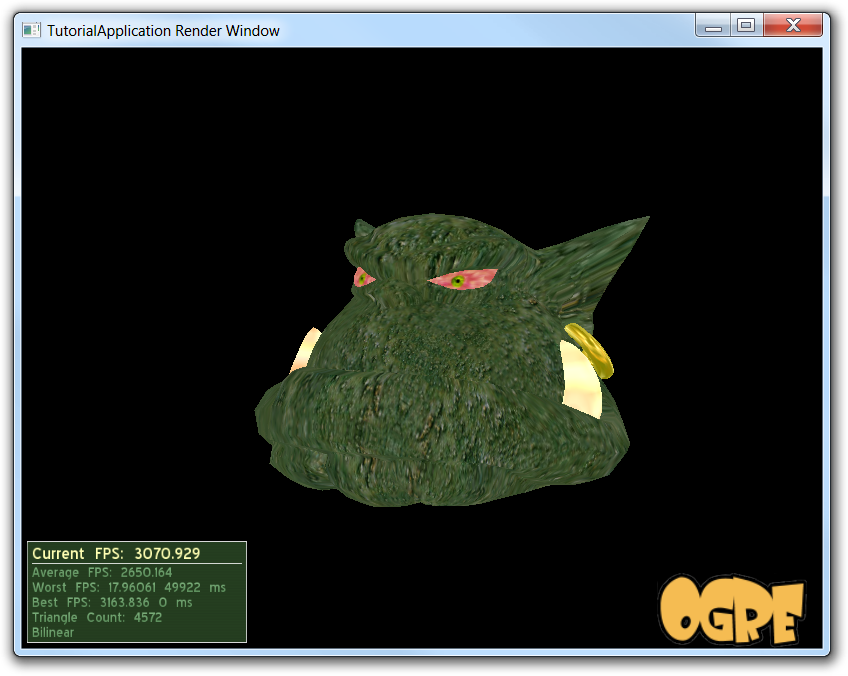
\includegraphics[width=7cm]{Images/mogre_logo.png}
&
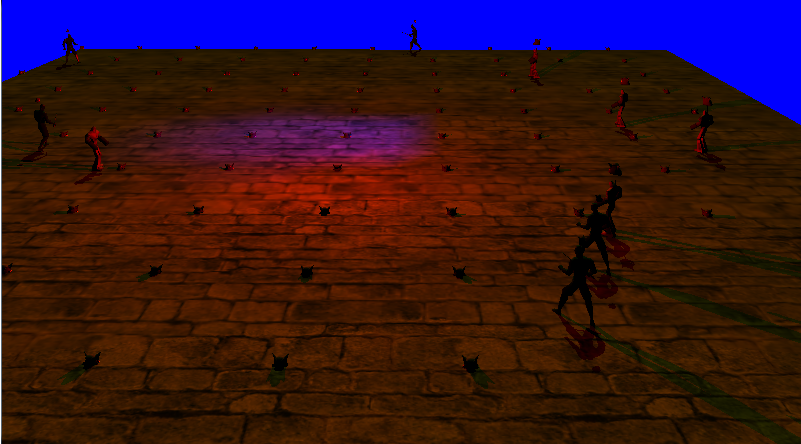
\includegraphics[width=8cm]{Images/mogre_capture.png}
\end{tabular}
\end{center}
